% !TeX spellcheck = en_US
\chapter{Approach}\label{ch:approach}

This chapter deals with the derivation of the solution approach for the comparison of the compression algorithms HDT and GraphRePair. First we will introduce some definitions and then we will discuss the concept of the solution approach.

\section{Definitions}

This chapter includes some basic definitions that will be used in the thesis.

\subsection{Compression Ratio}

One of the key metrics for a compressor is its compression ratio. The compression ratio depends on the input data and is defined as follows

\begin{align*}
	\text{compression ratio} = \dfrac{\text{compressed size}}{\text{original size}} \in (0,1]
\end{align*}

The compression ratio is typically in the $(0,1]$ interval, since the compressed data will not be larger than the original data (there are cases where this happens, but it does not happen in the compressors considered here). Obviously, the compressed data cannot have a size of 0 or less.

Normally the compression ratio is measured at the file size level (in byte). If a different measure is used, it will be mentioned at that point.

\subsection{(De-)Compression Time}

Another key metric of a compressor is its (de-)compression time. This metric also depends on the input data and indicates the run time needed for compression and decompression of the data, respectively. The run time is typically measured in milliseconds.

\section{Concept}

Fig.~\ref{fig:benchmark_overview} shows the aspects of a benchmark of two compressors. There are parameters that can be set during the evaluation (they start with $p$) and measures that represent the performance of the algorithms (they start with $m$).

The compressors get an input $p_{input}$, which in this case is in RDF graph. They each produce an output $m_{output}$, the compressed data. For compression and decompression there will be run times, which we call $m_{runtime} $. In addition, there are certain parameters $p_{alg}$ that can be set in the algorithms that change the behavior of the algorithm. \todo{hier kommt noch nicht performance von queries vor}

\begin{figure}[h]
	\centering
	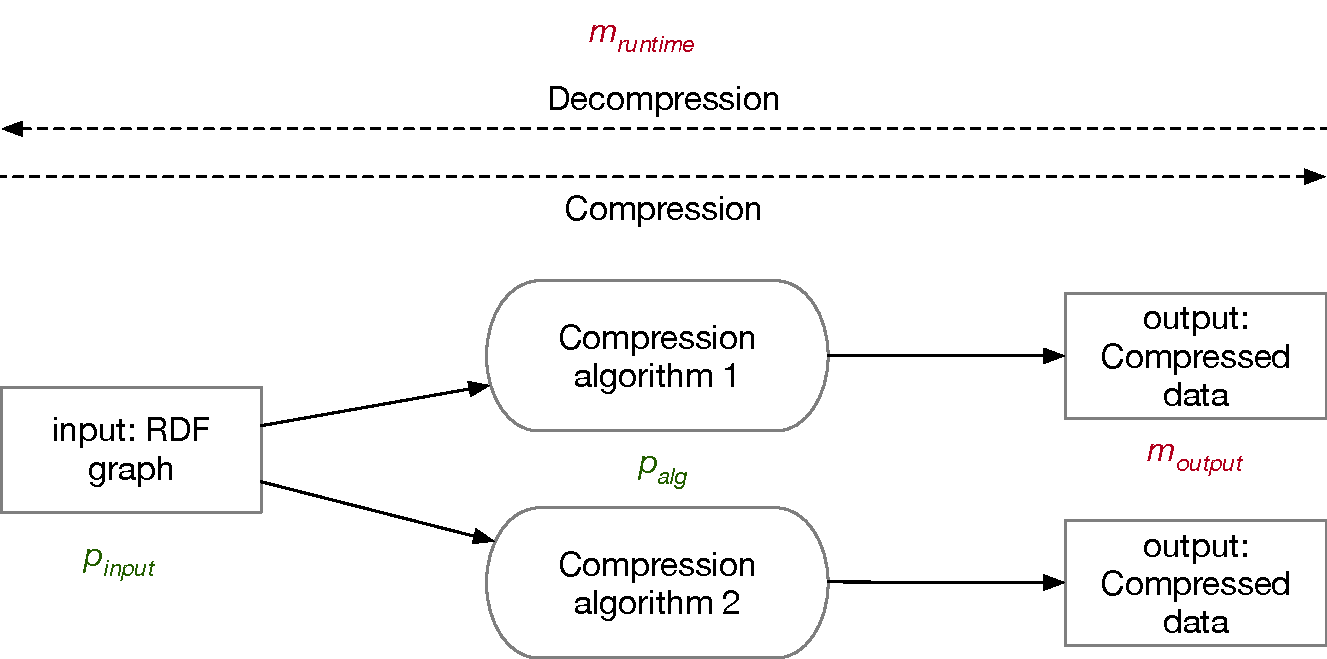
\includegraphics[width=1\textwidth]{figures/approach/Benchmark}
	\caption{The different aspects of a compression process. $p_{input},p_{alg}$ are parameters that can be changed. $m_{output},m_{runtime}$ are measures of the algorithm's performance.}
	\label{fig:benchmark_overview}
\end{figure}


